\vspace{3cm}

% \textbf{Àlex Giménez-Romero$^{1}$, Eduardo Moralejo$^{2}$, Manuel A.
%     Matías$^{1}$}

% \vspace{1cm}

% \begin{enumerate}
%     \small
%     \item Instituto de Física Interdisciplinar y Sistemas Complejos, IFISC
%           (CSIC-UIB), Palma de Mallorca 07122, Spain
%     \item Tragsa, Passatge Cala Figuera 6, 07009 Palma de Mallorca, Spain
% \end{enumerate}

% \vspace{1cm}

\textbf{Published as}

\vspace{0.5cm}

\fullcite{GimenezRomero2024}

\newpage
\section{Introduction}

Climate plays a pivotal role in shaping the distribution and dynamics of
agricultural pests and pathogens
\cite{Harvell2002,Lafferty2009,Bebber2013,Bebber2014,Delgado-Baquerizo2020},
with implications for global food security \cite{Fones2020, Ristaino}. As our
climate undergoes unprecedented changes due to anthropogenic activities,
agriculture faces multifaceted threats ranging from alterations in temperature
and precipitation patterns to increased frequency of extreme weather events
\cite{skendzic2021impact}. Such shifts create novel environments that may
favour the proliferation of certain pests or pathogens while posing challenges
to the survival of others \cite{Bebber2013, Dudney2021}. The consequences of
these changes extend beyond immediate agricultural landscapes, reverberating
through global food systems and posing significant challenges to the
sustainability and resilience of food production \cite{Ortiz-Bobea2021}.

Understanding the intricate relationships between climatic conditions, the
pathosystem components, and the subsequent epidemiological dynamics is
essential for developing effective strategies to mitigate and manage emerging
agricultural challenges, especially in the face of changing environmental
conditions. However, modelling disease epidemics is a complex task , as they
are emergent phenomena resulting from non-linear interactions between disease
components that also exhibit non-linear responses to changes in environmental
variables \cite{scherm1994global,garrett2011complexity,jeger2019epidemiology}.
Thus, while climate primarily determines the potential geographic range of each
organism in the pathosystem, the development of epidemic outbreaks depends on
favourable host-pathogen-vector-climate interactions that drive transmission
chains.

It has long  been recognised that ecological phenomena typically depend on
the scale of description,  particularly with regard to the effects of climate
\cite{Levin1992}. Climatic databases with finer spatial resolution are
continuously being developed with the goal of allowing more accurate
predictions \cite{Navarro-Racines2020}.  Some recent studies have shown that
the local climate experienced by individuals might deviate substantially from
regional averages, with implications for the population dynamics of a forest
herb \cite{Christiansen2024}. Likewise, the choice of climate data affects the
predictions of species distribution models (SDMs) \cite{Abdulwahab2022}. In
particular, the spatial resolution of the data can influence the predictions of
invasion risk for some species \cite{Dubos2023}.  It is therefore clear that
the resolution of climate data will have a significant impact on predicting the
risk of plant diseases and pests.

Among emerging pathogens \textit{Xylella fastidiosa} (Xf) is considered one
of the most dangerous phytopathogenic bacteria worldwide
\cite{Hopkins2002,EFSA_xf}. It is naturally transmitted by xylem sap-feeding
insects, such as sharpshooters and spittlebugs, and exhibits a broad host range
that encompasses economically important crops such as grapevines, citrus,
almonds and olive trees \cite{redak2004biology,EFSA_xf}. The consequences of Xf
diseases are devastating: about 200 million citrus trees are  infected annually
in Brazil \cite{Lindow2019}, there are	loses over \$100 million annually in
the grape industry in California  \cite{tumber2014pierce} and approximately
$21$ million olive trees have been killed by the bacterium on the Apulia region
in Italy  \cite{Sabelli2023}. Assuming massive spread throughout Europe, Xf has
been projected to potentially contribute up to \texteuro5.2 billion of annual
losses in the olive sector alone \cite{Schneider2020}. Overall, Xf diseases
pose a major threat to agrosystems worldwide, highlighting the need for precise
and predictive models to guide effective management practices.

Previous research has provided insights into the potential geographic range
of Xf subspecies through SDMs \cite{Bosso2016b, Godefroid2022}. These models,
however, have led to overestimates of risk by failing to account for the
distribution and abundance of potential vectors necessary for disease
transmission  \cite{Godefroid2022_vector}.  A quite different approach to
mapping the risk of Pierce's Disease of grapevine has been developed based on
climate-driven epidemiological models with the option to integrate vector's
distribution information and the specificity of the Xf subsp.
\textit{fastidiosa} strain responsible for the disease,
(hereafter \xf{}) \cite{GimenezRomero2022_CommsBio}. This model correctly
identifies areas in the United States with recurrent  PD outbreaks and
forecasts increasing epidemic risk in Mediterranean islands and coastlines
with ongoing climate change.

Although risk maps based on hourly temperature data from the ERA5 have
allowed fine adjustments in the calibration of the thermal response to Xf
infection, these achievements have entailed losses in spatial resolution (0.1º
spatial resolution) \cite{GimenezRomero2022_CommsBio, munoz2019era5land}. Such
limitation is particularly significant when dealing with vector-borne plant
diseases like PD, where the interactions between the pathogen, vector, and host
plants exhibit non-linear responses to climatic conditions. Subtle variations
in temperature, humidity, or precipitation at the local scale thus can have
profound effects on the reproduction and life cycles of the organisms involved
and, hence, on the dynamics of disease transmission.

Topographical heterogeneity is a recognised issue in invasion biology, but
has received little attention in crop science.	Vineyards are increasingly
located in valleys, ridges, hillsides and riverbanks usually with altitudinal
and microclimatic gradients in short transects.  They are therefore a
remarkable example of  a crop subject to scaling problems when studying
ecological or epidemiological processes at  regional and global scales.  In
this work, we address this spatial resolution limitation by modelling the risk
of PD  using high-resolution climate data from the CHELSA dataset
\cite{Karger2017}. The study period was deliberately chosen  to include real
data on temperature increases due to ongoing climate change.  Our study shows a
greater global risk of PD and a higher rate of risk increase, underscoring the
urgency of reevaluating global strategies to prevent the spread of the pathogen
with international trade in plant diseases.

\section{Results}

\subsection{Global differences in  PD risk between coarse and fine-grain
    climate data}

We computed the risk of PD using the previously developed climate-driven
epidemiological model in \cref{ch:commsbio} \cite{GimenezRomero2022_CommsBio}
coupled with the CHELSA dataset \cite{Karger2017}, which features key climate
variables (e.g. temperature and precipitation) at a high spatial resolution of
1 km and daily temporal resolution covering the period 1979-2016. The resulting
spatial and temporal patterns of disease risk in the main wine-growing regions
were compared with the previous risk projections derived from the ERA5 dataset
\cite{munoz-sabater_era5-land_2021} in \cref{ch:commsbio}, characterised by an
intermediate  spatial resolution of 10 km  and hourly temporal resolution
\cite{GimenezRomero2022_CommsBio}. Risk projections in Europe use the
climatic suitability, $s$, of the main European vector, \textit{P. spumarius}
(see Methods), while for the rest of the world it is assumed that there are no
risk-limiting effects due to the vector  ($s=1$), but only due to climatic
conditions.

When contrasting model results derived from high- and medium-resolution
data for the latest available time (2016), the disparity in risk projections
extends beyond regional differences, showing a global increase in risk indices
across wine-growing areas (\cref{fig:risk_indices_dif,fig:ERA5_vs_chelsa}).
Overall, these increases
(\cref{fig:risk_categories_dif}) in the extension of PD risk areas ranged from
100,000 to 1 million km$^2$ across viticulture regions worldwide. Transitions
from no-risk to risk zones covered an area one order of magnitude larger than
those in the opposite direction --from risk to no-risk
(\cref{fig:risk_categories_dif,tab:risk_category_dif}). In total, a surface of
4.6 million km-2 changed its risk category with the CHELSA database,
representing about a 16\% of the land area studied. In contrast, the largest
decreases in the risk indices occurred mainly in the Southern Hemisphere,
although with few exceptions most of these decreases remained within the risk
zones (\cref{fig:risk_indices_dif}), while similar land expansions were
observed to  increase their risk category (low to moderate or moderate to high)
(\cref{fig:risk_categories_dif,tab:risk_category_dif}). The largest changes in
risk indices occur in ecotones on both sides of the $r=0$ line, as is clearly
seen in the south-eastern United States, in coastal areas (e.g., southern
Australia and northern California) due to higher resolution that better
distinguishes between land and coast, and finally in the river valleys and
slopes of mountain systems
(\cref{fig:risk_categories_dif,tab:risk_category_dif}).

Next, we compared the temporal progression of the area at risk using both
high and mid-resolution data over the entire available time span (1986-2016),
considering that the risk for each year is computed based on the preceding
seven years. We found a notable global surge in the rate increase of the area
at risk within viticulture zones worldwide, practically doubling previous
estimates (\cref{fig:area_at_risk}). These results point to an
accelerated
pace at which the risk of PD is growing, compatible with the predictions of
different global warming scenarios \cite{GimenezRomero2023_PD}.

\begin{table}[H]
    \caption{Changes in Pierce's Disease Risk Zones in Different Viticulture
        Regions. The table illustrates transitions between risk and no-risk
        categories,
        as well as transitions among risk categories, highlighting the dynamic
        shifts
        in risk patterns across viticulture areas in Europe, the USA, South
        Africa,
        South America, and Australia. Risk increase refers to changes from low
        to
        moderate risk or from moderate to high risk. Likewise, risk decrease
        refers to
        changes from moderate to low risk or high to moderate risk.}
    \label{tab:risk_category_dif}
    \resizebox{\textwidth}{!}{%
        \begin{tabular}{lccccc}
            \hline
                                                 & \textbf{Europe}       &
            \textbf{USA}                         & \textbf{South Africa} &
            \textbf{South America}               & \textbf{Australia}
            \\ \hline
            \textbf{Risk to no-risk (km$^2$)}    & 1.91e+04
                                                 & 3.93e+04
                                                 & 2.26e+04
                                                 & 2.49e+05
                                                 & 5.81e+04
            \\
            \textbf{Transition to risk (km$^2$)} & 6.37e+04
                                                 & 1.37e+05
                                                 & 5.53e+04
                                                 & 3.79e+04
                                                 & 8.49e+04
            \\
            \textbf{Risk decrease (km$^2$)}      & 3.58e+04
                                                 & 1.46e+05
                                                 & 3.56e+05
                                                 & 1.76e+05
                                                 & 1.28e+06
            \\
            \textbf{Risk increase (km$^2$)}      & 6.28e+04
                                                 & 2.37e+05
                                                 & 1.05e+05
                                                 & 1.50e+05
                                                 & 1.55e+05
            \\
            \textbf{No risk to risk (km$^2$)}    & 2.04e+05
                                                 & 2.36e+05
                                                 & 2.77e+05
                                                 & 1.90e+05
                                                 & 2.15e+05
            \\
            \textbf{Total changes (km$^2$)}      & 3.85e+05
                                                 & 7.95e+05
                                                 & 8.15e+05
                                                 & 8.03e+05
                                                 & 1.79e+06
            \\ \hline
        \end{tabular}
    }
\end{table}

\begin{figure}[H]
    \centering
    \includegraphics[width=0.8\textwidth]{Figures/ERA5_vs_CHELSA_dif.pdf}
    \caption{Difference in risk projections based on CHELSA
        (high-resolution, 1 km) and ERA5 (mid-resolution 10 km) datasets in
        global
        viticulture areas. (A) Europe (B) South America (C) United States (D)
        Australia
        (E) South Africa.}
    \label{fig:risk_indices_dif}
\end{figure}

\begin{figure}[H]
    \centering
    \includegraphics[width=\textwidth]{Figures/ERA5_vs_CHELSA_zones.pdf}
    \caption{Changes in risk categories between CHELSA (high-resolution, 1
        km) and ERA5 (mid-resolution 10 km) projections in global viticulture
        areas.
        (A) Europe (B) South America (C) United States (D) Australia (E) South
        Africa.
        Risk category increase refers to changes from low to moderate risk or
        from
        moderate to high risk. Likewise, risk category decrease refers to
        changes from
        moderate to low risk or high to moderate risk.}
    \label{fig:risk_categories_dif}
\end{figure}

\subsection{Pierce's Disease risk surges in previously unresolved
    microclimates}

River valley vineyards are renowned  for their high quality wines, such as
Douro, Napa and Rhone and many others. It is therefore important to understand
the risk of  PD with climate change at	a more detailed level. In our analysis,
we have identified rivers and valleys as specific relief areas where a greater
increase in PD risk is observed when employing CHELSA’s finer- scale climate
data (\cref{fig:microclimates}).

\begin{figure}[H]
    \centering
    \includegraphics[width=0.9\textwidth]{Figures/ERA5_vs_CHELSA_rivers.pdf}
    \caption{Effect of microclimatic conditions of rivers and valleys on
        Pierce's Disease of grapevines. Comparison of the risk predicted using
        ERA5
        mid-resolution dataset (A,C,E) and CHELSA high-resolution dataset
        (B,D,F).
        (A-B) North-western Iberian Peninsula. (C-D) Sourthern France and
        North-eastern
        Spain. (E-F) Western United States. Black dots represent grapevines
        (\textit{Vitis vinifera}) presence data obtained from GBIF (see
        Methods).}
    \label{fig:microclimates}
\end{figure}

In some important wine-growing areas of
southern Europe, we observed an abrupt emergence of risk zones previously
classified as no-risk when using lower resolution climate data
(\cref{fig:microclimates}). Such pronounced differences in risk patterns are
highlighted for example in the fairly steep valleys and hillsides along the
Douro River in Portugal, where the specific microclimatic conditions were
previously obscured by the coarser resolution of the ERA5 data. These findings
are particularly significant for PD,  as vineyards are often located in close
proximity to rivers or valleys and their surroundings, creating microclimates
that attenuate cold winters (black dots in (\cref{fig:microclimates})). A
gradual increase in the climatic suitability for PD in some river basins may
thus favour the spread of the pathogen from coastal  to interior areas of the
continents, allowing interconnection between areas that would otherwise remain
isolated. Coastal areas close to cool water masses may also undergo an increase
in risk  when using higher resolutions data, as exemplified in California
(\cref{fig:microclimates} e,f).

\begin{figure}[H]
    \centering

    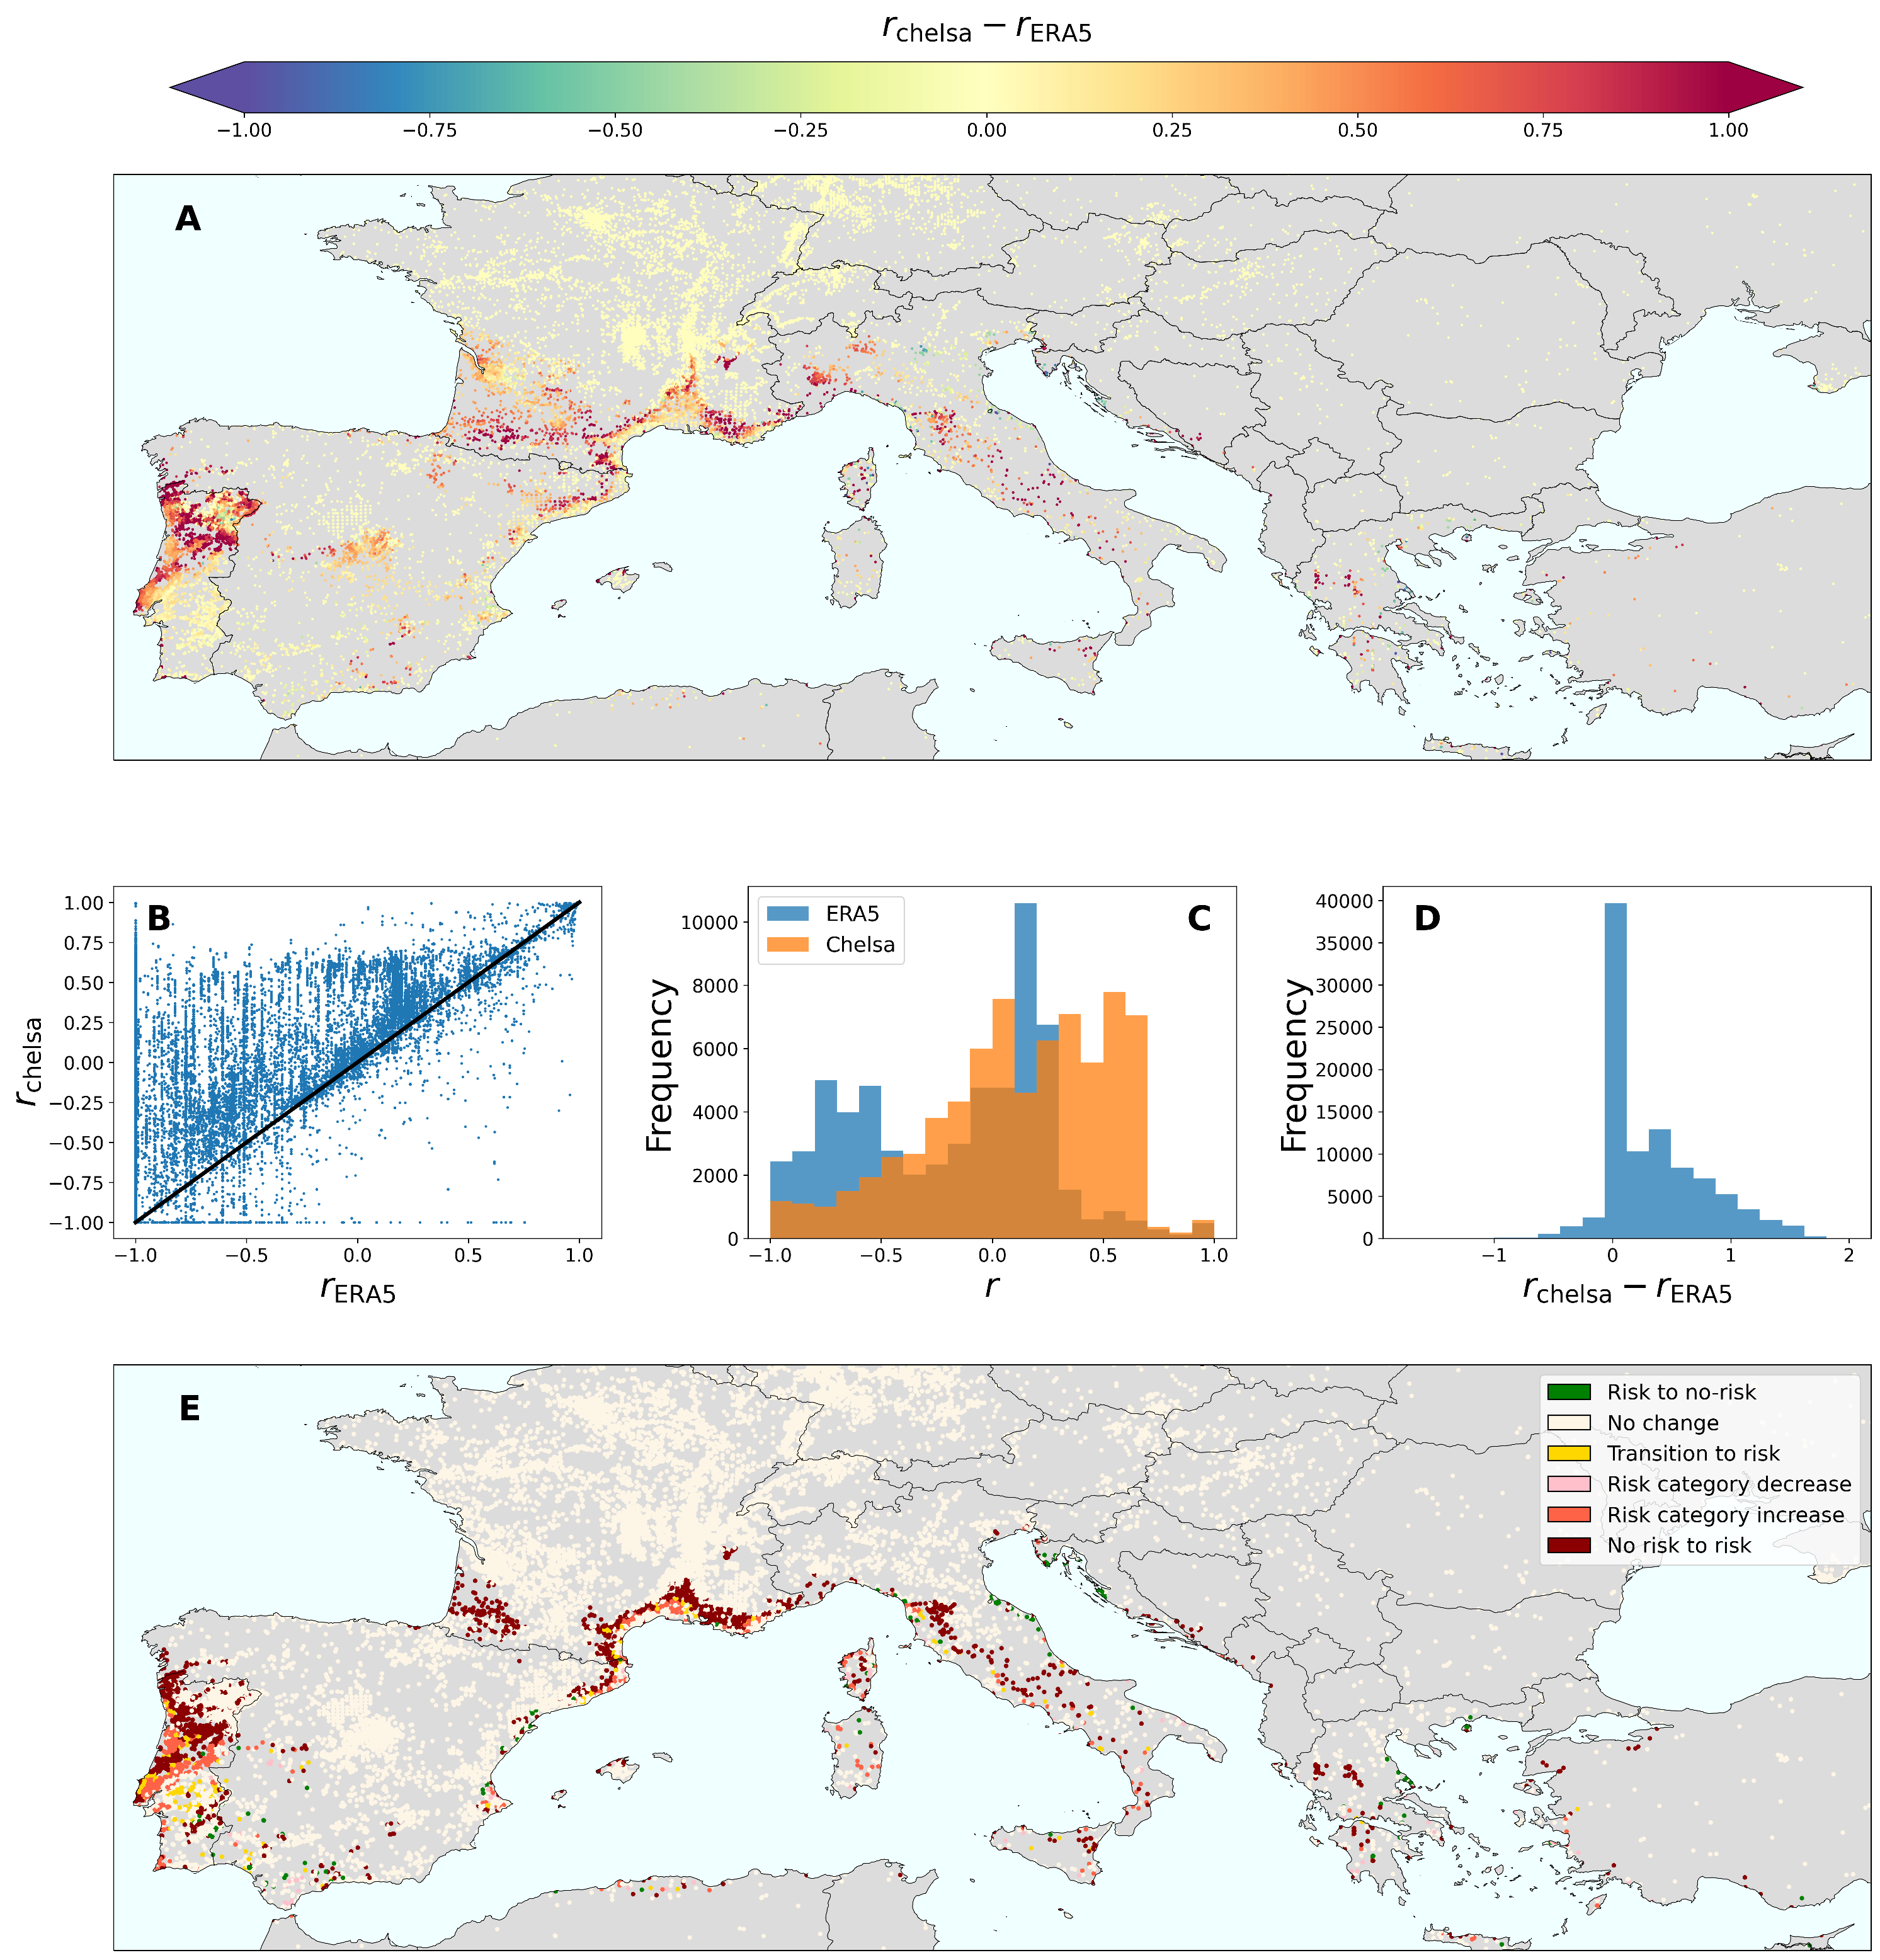
\includegraphics[width=0.9\textwidth]{Figures/risk_difference_vineyards.pdf}
    \caption{Impact of high-resolution climate data on the risk of Pierce's
        Disease for grapevines worldwide. (A) Difference in risk indices in
        Europe,
        which accounts for the 96\% of the points in the dataset. (B)
        Comparison of the
        risk indices derived from CHELSA and ERA5 datasets. Points with perfect
        agreement would lie in the solid black diagonal curve. (C) Histogram of
        risk
        indices derived from ERA5 (blue) and CHELSA (orange). (D) Histogram of
        the
        differences in risk indices between CHELSA and ERA5 datasets. (E)
        Changes in
        risk categories when using high-resolution climate data (CHELSA) with
        respect
        to mid-resolution data (ERA5). Risk category increase refers to changes
        from
        low to moderate risk or from moderate to high risk. Likewise, risk
        category
        decrease refers to changes from moderate to low risk or high to
        moderate risk.}
    \label{fig:risk_dif_vid}
\end{figure}

Finally, to obtain a comprehensive assessment of the impact of
microclimatic conditions on the risk of PD establishment, we collated a dataset
of over 100,000 \textit {Vitis vinifera} presence locations worldwide from GBIF
\cite{GBIF}, with a predominant concentration of points from Europe
(\cref{fig:vid_locations}). Each data point was assigned a risk index
based on
the ERA5 and CHELSA projections, respectively, using the nearest pixel from
each database.

This approach revealed an increase in the risk indices
associated with the vine locations (\cref{fig:risk_dif_vid} A-D), mostly
showing shifts towards higher risk indices (\cref{fig:risk_dif_vid} A,E) from
no risk to risk, or increases in risk category (low to moderate or moderate to
high), while a negligible number of points decreased in risk category
(\cref{fig:risk_dif_vid} E). Such behaviour was common to all key viticulture
regions studied, although the extent of increases differed between continents,
with substantial expansion of vineyard areas at risk in Europe and South Africa
(\cref{tab:risk_increase_vid}). Overall, our results emphasise the global
relevance of microclimatic conditions in influencing the risk landscape for PD
in viticultural areas (\cref{tab:risk_increase_vid}).

\begin{table}[H]
    \centering
    \caption{Comparison of grapevine presence locations at risk in key
        viticulture regions using CHELSA and ERA5 datasets}
    \label{tab:risk_increase_vid}
    \resizebox{\textwidth}{!}{%
        \begin{tabular}{lccc}
            \hline \hline
                                   & \multicolumn{1}{l}{\textbf{Nº points}}
                                   & \multicolumn{1}{l}{\textbf{risk
            CHELSA (\%)}}          & \multicolumn{1}{l}{\textbf{risk ERA5
                    (\%)}}
            \\ \hline
            \textbf{Europe}        & 96102
                                   & 41.2                                   &
            21.8
            \\
            \textbf{USA}           & 792
                                   & 69.8                                   &
            66.3
            \\
            \textbf{South Africa}  & 36
                                   & 47.2                                   &
            5.6
            \\
            \textbf{South America} & 112
                                   & 77.7                                   &
            74.1
            \\
            \textbf{Australia}     & 186
                                   & 51.6                                   &
            45.7
            \\ \hline \hline
        \end{tabular}%
    }
\end{table}

\section{Discussion}

Our study sheds light on the  relevance of the spatial scale of observation
in the intricate interplay between microclimatic conditions and the risk of PD
for grapevines on a global scale. The use of high-resolution climate data
reveals previously unrecognised local areas with microclimates conducive to the
establishment of PD worldwide. Contrary to the simplistic assumption that
higher resolution data might yield only marginal distinctions at regional
levels, our study demonstrates that slight variations in climate data at local
scales can lead to a global surge in disease risk. These increases  not only
affect the spatial distribution of risk, but also its temporal dimension, as
suggested by the rate of increase in the surface area at risk. In the case of
PD, we show that this rate nearly doubles when high-resolution climate data is
considered compared to previous estimates obtained with mid-resolution data.
Thus, our findings indicate a critical need for the use of local or
high-resolution climate data in the assessment of disease risk, especially in
areas characterised by diverse topography and even when only attempting to
global estimates.

Such observed differences arise from the non-linear nature of disease
dynamics and the response of the pathosystem components to environmental shifts
\cite{scherm1994global,Dudney2021}. Therefore, models dependent on broader
climate data may not capture the complexities of microclimates, resulting in an
underestimation of disease risk.  While this is not inherently negative,
recognising these limitations helps to assume such risk estimates as a
conservative lower bound until proven otherwise . Acknowledging these
constraints is crucial for refining our understanding of disease dynamics and
ensuring that our risk assessments are sufficiently cautious in the absence of
more reliable data. Likewise, data coarsening procedures should be avoided, if
possible, when modelling climate-driven disease dynamics, even in spite of
computational efficiency. This recommendation applies not only to disease risk
predictions but to all those in which non-linear functions depending on climate
variables are present, such as species distribution models or phenological
models \cite{menzel2006european}.

Despite the valuable insights gained,  our analysis heavily relies on the
quality and resolution of the climate data from the CHELSA dataset
\cite{chelsa-climatologies-2021}. While this dataset offers information at a
high spatial resolution, the temporal dimension is limited to a daily
frequency, which forces to apply an approximation to infer hourly data.
Furthermore, the data may still be subject to biases or uncertainties inherent
to the nature of the methodology employed in their construction . On the other
hand, vector presence data is only accurately obtained for Europe, while an
homogeneous presence is assumed in other viticulture areas. Additionally, the
study primarily focuses on the effect of temperature conditions and the
presence of potential vectors to determine the risk of	Xf establishment, which
may not encompass all possible contributing factors. Other variables, such as
soil characteristics or vineyard management practices were not explicitly
considered in this analysis, leaving room for additional complexities in the
disease dynamics. Furthermore, the study predominantly examines the risk at a
global scale, and the applicability of the findings to specific local contexts
may vary.

Future research should aim to address the aforementioned limitations and
provide a more comprehensive understanding of the multiple interactions
influencing PD development  in viticulture regions. Other factors influencing
disease spread, such as human behaviour, land use changes, and ecological
shifts, should also be explored, offering a more comprehensive and holistic
view of the interplay between environmental conditions and disease
vulnerability. The acceleration in the rate at which the risk of PD is growing
calls for more research into control strategies to mitigate its impact on
grapevine crops worldwide.

Although PD is currently restricted to North America and recently
introduced in Taiwan \cite{su2013pierce}, Mallorca (Balearic Islands, Spain)
\cite{gomila2019draft,moralejo2019insights} and Israel
\cite{zecharia2022xylella}, since the mid-1990s climatic conditions are
increasingly conducive to the establishment of PD in southern Europe
\cite{GimenezRomero2022_CommsBio}. For example, with the increase in the
resolution of
climate data our model predicts  the recent detection of PD in Portugal
\cite{loureiro2023xylella}, which was not anticipated using the ERA5 data
\cite{GimenezRomero2022_CommsBio}. In a short time, it is foreseeable that
there will
be more epidemic outbreaks in vineyards in southern Europe if the entry of
infested plants is not controlled. This not necessarily have to be vines but
can also include other plants such as almond trees or ornamental plants
\cite{moralejo2020phylogenetic}.

Overall, our study contributes to the growing body of knowledge on the
impact of climate on agricultural pests and pathogens, emphasising the
importance of considering microclimatic conditions for a more deep
understanding of disease dynamics. Future research should focus on developing
comprehensive models that integrate high-resolution climate data, considering
both the global and local factors that influence disease dynamics. This
holistic approach will enable a more accurate prediction of disease risk,
allowing for the development of targeted management strategies and the
enhancement of global food security.

\section{Methods}

\subsection{Climate data}

Climate data was downloaded from two datasets for our analysis: the ERA5
dataset \cite{munoz-sabater_era5-land_2021, munoz2019era5land} and the CHELSA
dataset \cite{Karger2017, chelsa-climatologies-2021}. ERA5 offers
mid-resolution climate data with a spatial resolution of 10 km and hourly
temporal resolution, while CHELSA provides high-resolution data with a spatial
resolution of 1 km and daily temporal resolution. Both datasets exhibit global
coverage and encompass crucial climate variables, such as temperature and
precipitation. For our simulations, we used the mean hourly temperature data
from ERA5 dataset and the maximum and minimum daily temperature data from
CHELSA dataset.

\subsection{Vector climatic suitability}

Vector climatic suitability data was obtained from \cite{Godefroid2022}, in
which a Generalised Additive Model (GAM) is employed to calibrate the
relationship of \textit{P. spumarius} global occurrence with moisture index and
maximum temperatures during summer index estimated from 1979 to 2013 using the
CHELSA dataset.

\subsection{Vineyard data}

To assess the risk of Pierce's Disease in locations where grapevines are
present, we collected a comprehensive dataset of over 100,000 \textit{Vitis
    vinifera} presence data records from the Global Biodiversity Information
Facility (GBIF) \cite{noauthor_what_nodate,GBIF}. We note that while the
dataset spans the globe, 96\% of the points are located in Europe
(\cref{fig:vid_locations}).

\subsection{Model adaptation to daily temperature data}

We used the model developed in \cref{ch:commsbio}
\cite{GimenezRomero2022_CommsBio}, in which MGDD and CDD metrics were defined
using hourly temperature data (\cref{eq:MGDDdef,eq:CDDdef}).However, the CHELSA
dataset only provide daily granularity. To overcome this limitation, we use a
basic sinusoidal extrapolation relating maximum and minimum daily temperature
to hourly temperatures,
\begin{equation}
    T_h=\frac{T_{max}+T_{min}}{2} + \frac{T_{max}-T_{min}}{2}\sin(w\cdot h)
    \ ,
\end{equation}
with $w=2\pi/24$ and $h$ ranging from $0$ to $23$. This approximation was
validated in \cref{ch:xf_climate_change} \cite{GimenezRomero2023_PD} with data
from national meteorological stations in Spain (AEMET) using several locations
and years, showing no differences between the use of hourly or daily
temperatures to estimate MGDD and CDD. Similarly, the use of the approximation
was validated across Europe using EURO-CORDEX data.